% \documentclass[onecolumn,doublespacing]{risa}
\documentclass[review,3p,times,onecolumn,sort&compress,12pt]{elsarticle}
% \documentclass[review]{elsarticle}

\usepackage[figuresright]{rotating}
\usepackage{tabularx}
\usepackage{longtable}
\usepackage{array}
\usepackage{graphicx}
\graphicspath{ {./fig/} }
\usepackage{afterpage}
\usepackage{enumitem}
\usepackage{multirow}
\usepackage{moreverb,url}
\PassOptionsToPackage{hyphens}{url}\usepackage{hyperref}
\usepackage[american]{babel}
\usepackage{csquotes}
\usepackage[
    style=apa,
    backend=biber,
    sortcites=true,
    maxcitenames=2,
    sorting=nyt,
%    isbn=false,
%    url=false,
%    doi=false,
%    eprint=false,
    hyperref=false,
    backref=false,
%    firstinits=false,
]{biblatex}
\let \citeNP \cite
\let \citeA \textcite
\let \cite \parencite

\newcolumntype{L}[1]{>{\raggedright\let\newline\\\arraybackslash\hspace{0pt}}m{#1}}
\newcolumntype{C}[1]{>{\centering\let\newline\\\arraybackslash\hspace{0pt}}m{#1}}
\newcolumntype{R}[1]{>{\raggedleft\let\newline\\\arraybackslash\hspace{0pt}}m{#1}}

\makeatletter
\AtEveryCitekey{\ifnameundef{shortauthor}{}{\def\cbx@apa@ifnamesaved{\@firstoftwo}}}
\makeatother

% \bibliographystyle{model5-names}\biboptions{authoryear}


\DeclareLanguageMapping{american}{american-apa}

\bibliography{references}

\journal{Transportation Research Part D}

\begin{document}

\begin{frontmatter}

\title{The Resilience of Access to Urban Services: Hazard vulnerability, recovery, \& equity}

%% Group authors per affiliation:
% \author{Elsevier\fnref{myfootnote}}
% \address{Radarweg 29, Amsterdam}
% \fntext[myfootnote]{Since 1880.}

%% or include affiliations in footnotes:
% \author[mymainaddress,mysecondaryaddress]{Elsevier Inc}
% \ead[url]{www.elsevier.com}

% \author[mysecondaryaddress]{Global Customer Service\corref{mycorrespondingauthor}}
% \cortext[mycorrespondingauthor]{Corresponding author}
% \ead{support@elsevier.com}

% \address[mymainaddress]{1600 John F Kennedy Boulevard, Philadelphia}
% \address[mysecondaryaddress]{360 Park Avenue South, New York}

% \author[Anderson]{Mitchell J Anderson$^{1,2}$\affiliation{Civil and Natural Resources Engineering, University of Canterbury, New Zealand}
% %
% Dai A F Kiddle$^{1}$
% %
% Tom M Logan$^{1,2}$\affiliation{The Cluster for Community and Urban Resilience, University of Canterbury, New Zealand}}

\begin{abstract}
To understand and improve community resilience we must be able to evaluate and understand the direct and indirect role of the transportation network.
This requires moving beyond a fixation on network functionality and towards an approach that can evaluate whether the network is truly serving the community’s needs.
In this paper, we present such an approach.
With the understanding that sufficient and equitable access to amenities is key to community resilience we leverage OpenStreetMap data and routing algorithms to simulate road and service closures under a range of hazard scenarios.
We illustrate this approach in three case studies.
Under different hazard scenarios, we repeatedly update the network based on simulated damage and restoration options to understand the sufficiency and equity of access before, during, and after a hazard event.
Ultimately, this information can support planners and policy-makers to better prepare their communities and respond equitably and efficiently when a disaster occurs.
\end{abstract}

\begin{keyword}
Resilience; Transport networks; Equity; Accessibility; Urban planning; Natural hazards
\end{keyword}

\end{frontmatter}


%%%%%%%%%%%%%%%%%%%%%%%%%%%%%%%%%%%%%%%%%%%%%%%%%%%%%%%%%%%%%%%%%%%
% INTRODUCTION
%%%%%%%%%%%%%%%%%%%%%%%%%%%%%%%%%%%%%%%%%%%%%%%%%%%%%%%%%%%%%%%%%%%

\section{Introduction}
% Context
% This paper is about the critical but indirect role of the transportation network in community resilience.
% Due to the indirect influences/implications/.., the transportation network plays a critical role in community resilience.
The transportation network's role in community resilience is perhaps more critical than generally understood.
This is due to the externalities and indirect effects that are caused by a disruption within the network. 
These effects are observed time and again in the wake of most disasters within a community, city, or country.
% Indonesia
An example is seen during the 2018 earthquake and tsunami in Indonesia.
This event, by severely damaging the horizontal and vertical infrastructure, resulted in thousands of young children losing access to their education \cite{Claire_Garmirian2019-lv}. 
Many of these children were still unable to return to school two years later, causing severe delays in the development of Indonesia's youth \cite{gibbs2019delayed}.
% Katrina
Hurricane Katrina in 2005 provides another example. 
The direct impacts of the event included the closure of many roads and services.
While roads were reopened promptly after the retreat of the water and clearance of debris, many services, such as supermarkets, did not reopen for many years after the event.
This impact to the transportation network and distribution of operable supermarkets meant that some poorer residents had to take three buses to their nearest supermarket for more than eight years after the event \cite{Netter_2016-zp}.
% Segway to community resilience?
Events like these make us question what could have been done to make these communities more resilient.

% Community Resilience
The resilience of a system is fundamentally related to its capacity to withstand, prepare for, recover from, and adapt or transform following hazards \cite{Bene2012-mx, Meerow2016-definingRes, GillespieMarthaler2019-ak,Cutter2016-xv}.
Traditionally, resilience is considered through two disparate lenses: community capacity \cite{Cutter2014-lr, Zautra2008-nc} and infrastructure functionality \cite{lin2018empirical, Cutter2014-lr}.
The former approach classically requires identifying the qualities that a community requires so it can withstand, prepare for, recover from, and transform after a shock \cite{Cutter2010-ee, Cutter2016-xv, Cutter2014-lr, Sherrieb2010-lk}.
Well-known examples of this community capacity view of resilience are seen within resilience indicators such as DROP \cite{Cutter2008-if}, BRIC \cite{Cutter2014-lr}, and SOVI \cite{Cutter2003-xi}.
The other view of resilience centers on infrastructure functionality.
The focus is on buildings, transportation, electricity, and other infrastructure with a primary view to avoid or mitigate damage, and quickly remedy any loss of functionality \cite{Bruneau2003-lk, Barker2013-uf, Curt2018-mm, Guidotti2016-hc, Hosseini2016-ae, Haimes2009-oi}.
As a result of their work, the resilience function or recovery curve has become a widely used and understood quantification of infrastructure resilience \cite{Bruneau2006-jg, Sharma2018-uh}, with recent work demonstrating how to utilise resilience functions to optimise recovery.
While both approaches are critical to our understanding of resilience, they fail to address the question at their interface: 
how does a community foster the capacities necessary for resilience and how can infrastructure enable these capacities before, during, and after a disruption?

% Access
Critical to fostering community resilience is accessibility to day-to-day services \cite{logan2020reframing}.
Health care, education, food, emergency service, cultural, and recreational centers are examples of amenities that are critical to the livability, safety, and cohesion of a community \cite{Contreras2017-wn, Dempsey2011-sv, Talen2003-iy, winter1997coordinating, logan2020reframing, unesco-jn}.
A lack of access to these amenities can transform a short-term disruption into a long-term social disaster, as seen in New Orleans and Indonesia \cite{watt-ht, Netter_2016-zp, Contreras2017-wn}.
However, in the presence of sufficient and equitable access, communities begin to foster a range of positives capacities such as community cohesion, social capital, and sense of place \cite{Jennings2019-jk, Forrest2001-wz}.
These qualities, in turn, enhance a community's ability to withstand, prepare, and act following a disruption; thus improving the community's resilience.


% This integrates the properties of both infrastructure functionality and community capacity.
% It does this by quantifying residents accessibility to essential services such as  \cite{logan2019evaluating}.
Therefore, it is important for us to ensure our communities are designed with access to the services they need.
However, while some communities have suitable access to amenities, many do not \cite{Logan2021-ineq}.
Large segments of our communities, in both developed and underdeveloped nations, are living within food deserts, health care deserts, and areas without access to other essential services \cite{Beaulac2009-sf}.
Because people with better access to resources are reported to have higher resilience \cite{Frazier2013-wd}, in the event of a disaster or disruptive event it is the access poor communities that are disproportionately impacted.

As a result, planners need to consider not just access, but equity in that access \cite{Dempsey2011-sv}.
That is, while access is necessary to a resilient community, it is not sufficient: the access itself must also be equitable.
Equitable access requires that people not only have the same (equal) access, but a level of access appropriate for their unique needs \cite{Lucy1977-dt, Talen1998-mk}.
This equity of access is a form of distributional justice and is one of the pillars of environmental justice \cite{Low2013-yx}.

%transport
%The transportation network is so integrated into urban living that to make advances in knowledge within the urban environment we must be able to model the transport network and it's impacts.
Critical to equitable access to these services is an effective transportation network.
Transportation networks are a foundation of society, on which we depend for daily mobility, the transport of goods, and the ability to provide aid and repairs in post-disaster scenarios \cite{Mattsson2015-mg, Dalziell2001-un}.
% economic
So much so, that before the introduction of the internet, the transportation network influenced almost 100\% of the United States GDP \cite{Han2000-rn}.
In under-developed nations, the transportation network has been evaluated as the ``formative power to economic growth'' \cite{Hoyle1973-ms}.
% urban form, shaping cities
But economic influence is not the only impact that the transport system plays within society.
The transportation network lays the foundations around which we construct our cities.
Where done well, the transportation layout promotes active transport, vibrancy, safety, better well-being, and of course, equitable access \cite{Jacobs2016-ks}.

%segway into disruptions and risk
To enable the continuation of community function, the transportation network must be effective before, during, and after a disruptive event.
In the event of a disaster, the restoration of all other lifeline systems depends on the ability to move people and resources to the sites where damage has occurred \cite{Hopkins1991-ok}.
Therefore, the transportation network is the most important infrastructure lifeline within a city.
In the wake of a disaster, affected residents may struggle to be rescued, while the loss of access through a main arterial link can cause major economic losses for a community \cite{Dalziell2001-un}.
More generally, disrupted access leads to increases in travel time that impairs the ability of individuals to take part in their daily activities, including commuting; dropping off and picking up children from day-care/school; and shopping.
For businesses, the impacts can include delayed deliveries and supplies; loss of customers and manpower; and increases in freight costs \cite{Jenelius2012-vp}.
One example of disrupted access in a community was seen during the COVID-19 pandemic, residents of Pokeno, a small New Zealand town, were forced to travel 40km to their nearest available supermarket as a regional lock-down made it impossible for them to access their otherwise nearest supermarket \cite{Preston2020-fc}.
To avoid similar planning failures and unjust recovery efforts, much like that of New Orleans, we must promote considerations of access to services within scenario and resilience planning.

% Niche
While research has been completed to understand the reliability and resilience of transport networks, current assessments often neglect two things: the needs of the people that the network serves, and the broader objective of the network; which is to allow people to travel between destinations of interest.
Yet, the transport network is all-but redundant if there are no operable destinations.
Without considering the operability of destinations (fixation on network functionality) can lead to a distorted understanding of the impacts that a disruption has on access and community function.
% Previous work on disruption measures on access/transport
The work to date on the resilience of access or transport networks often deals in the following:

\begin{enumerate}
    \item The delegation of resources after a disaster to optimise the restoration process \cite{Sun2020-ln, Li2020-nq, Ozdamar2014-fh, Tuzun_Aksu2014-gq}
    \item High-level impact assessments of major transport links or very localised impact assessments on small complex networks \cite{Dalziell2001-un, Khademi2015-jq, Tuzun_Aksu2014-gq, Nicholson2007-zc, Jenelius2012-vp, Chang2001-bq, Bono2011-dk, Sohn2006-vg, Taylor2012-jw}
    \item Transport demand models for evacuation \cite{Tuzun_Aksu2014-gq, Cova1997-vl}
\end{enumerate}

Very few studies evaluate the impact of a network disruption at a city-wide level, let alone the impact on a communities ability to function and recover.
Within one recent study, we see the distribution of access evaluated over time as a city's supermarkets and service stations are made inoperable and slowly restored based on real-time data in the wake of a disaster \cite{logan2020reframing}.
However, this study only evaluates access change by removing and adding operable facilities as they are closed and reopened respectively, it does not consider changes to the transport network.
Another study evaluated the isolation potential of residents after a disruptive event by modelling changes to the transport network \cite{Bono2011-dk}. 
However, this study did not quantify access to different services, only identified where potentially isolated residents are. Therefore, it does not evaluate the resilience of a community or its access network.

% Contribution
%% Isolation
The main contribution of this paper is to improve the understanding of the role that the transportation network plays in community resilience and to explore an approach to evaluate the direct and indirect impacts following a disaster.
Specifically, measuring the change in a community's ability to function through the change in accessibility and associated equity after a sudden disruption in the transport network and distribution of operable services.
We do this by evaluating the performance and equity of access to health care, education, and supermarket facilities within a city under a business as usual scenario as per \textcite{Logan2021-ineq}.
This is done before simulating a hazard scenario on the city which identifies a set of transport network segments and services that are no longer usable.
These direct hazard impacts are then used within the re-evaluation of the city's access performance and equity.
This allows for the evaluation of the vulnerability and resilience of a city's access.
Moreover, it allows for a better understanding of the residents within a community that will be affected by the changes in their surrounding networks.
We demonstrate this approach under different hazard types within three cities; (1) Seattle (WA, USA), due to liquefaction damage from a simulated earthquake event; (2) Houston (TX, USA), due to inundation damage from a simulated hurricane event; and (3), a multi-hazard event in Christchurch (New Zealand) due to inundation and liquefaction damage from a simulated earthquake-induced tsunami event.
The three case studies provided are used to display, (1) the simulated change in access distribution and associated equity across different demographic groups with inclusions of uncertainty; (2) areas and demographic groups prone to isolation from different service types; and (3), the ability to use multi-criteria optimisation to aid decision-makers in the process of coordinating an equitable restoration program.
An interactive app demonstrating the process and our results are provided here: [Link redacted for blind review]


%%%%%%%%%%%%%%%%%%%%%%%%%%%%%%%%%%%%%%%%%%%%%%%%%%%%%%%%%%%%%%%%%%%
% METHOD
%%%%%%%%%%%%%%%%%%%%%%%%%%%%%%%%%%%%%%%%%%%%%%%%%%%%%%%%%%%%%%%%%%%

\section{Methodology}
Our goal is to evaluate the indirect impacts of a natural hazard on a community's transportation network.
Specifically, evaluate resident's access to essential services over time by quantifying the access before, during, and after a disruptive event.
The first step in this process is to quantify a city’s access to services under normal circumstances.
We do this by evaluating the network distance between a set of origin-destination (O-D) pairs \cite{logan2019evaluating,Logan2021-ineq}. 
Then, critical to understanding the impact of a hazard and the role of the transportation network and one of the major differences with previous work, is to model how this access changes during and after a natural hazard event.
We achieve this by simulating damage to both the transport network and buildings before running large scale O-D queries on the updated networks. 
Once we have determined the new distribution of access between residents, we then evaluate the equity and change in equity \cite{sheriff2020health, Logan2021-ineq}.
Finally, we look to network recovery with the use of isolation and equity of access to drive a multi-criteria optimisation process that can guide recovery plans. 
This guide to prioritising network restoration is determined by developing different network recovery pathways and evaluating the access, isolation, and equity throughout each one.
We can then create a prioritised ranking of roads and services to restore based on a multi-criteria greedy optimisation function which we then compare against a random recovery function. 
We elaborate on these steps in the following subsections.
Our code is available on GitHub: [redacted for blind review].

\subsection{Data Inputs and Processing}
Our approach requires the following data to be input: Origins (e.g., the location of the centroid of each neighbourhood block), destinations (the key services in the community, e.g., supermarkets), population and demographic data (Census), the transport network, and a hazard scenario.
We describe these in the following sections and list our case studies' data sources in Appendix A, \autoref{tab: data}.

\subsubsection{Origin and Destination Pairs}
To quantify access within a city we require the locations of origins and destinations of interest.
The set of origins generally represents the usual place of residence for people within the city.
When selecting origin points within a city there is a trade-off in the resolution used. 
Larger resolutions, i.e. census tracts, are computationally simpler but can underestimate distance and overlook access-poor residents \cite{logan2019evaluating}. 
We recommend using neighbourhood block centroids as origins. 
For computational efficiency, we limit origins to all census blocks, within the city, with at least one resident.

The destinations are the locations of services and/or amenities around and near the city. 
The selection of what type of destinations are included should be based on the needs and values of the community and, in practice, should be selected based on engagement with local governments and communities \cite{Simonsen2012-bj}.
Destinations within a 5km buffer of the city boundary are included to ensure that residents on the edge of the city were not arbitrarily misrepresented.
Care is necessary when sourcing the destination locations as errors (not uncommon in commercial, government, and VGI data \cite{Wong2017-it}) may result in a misrepresentation of the vulnerabilities within a community which, in turn, may lead to ineffective or even maladaptive interventions. 

Within our three case studies, we use three destination types: supermarkets, health care facilities, and primary schools.
The destination data was checked by visual comparisons with Google Maps and corrected as necessary to add or remove destinations.
The boundaries used are defined as the county boundaries in the USA (King and Harris counties for Seattle and Houston respectively) and the Christchurch City Council boundaries for Christchurch, New Zealand.

Once we have identified the set of origins and destinations we create a joint set of origin-destination (O-D) pairs, such that every origin is paired with every destination.

\subsubsection{Transport Network Data}
To calculate the network distance between the origin and destination pairs, we require the transport network.
We extract the transportation network from OpenStreetMap \cite{OpenStreetMap}.
However, when the shapefile is required for the exposure assessment we extract the same network using OSMNX \cite{Boeing2017-nf}. 
Consistent with the destinations, we extract the transport network that is within a 5km buffer of the city boundary to ensure routes are not restricted to find the nearest service.
We then use the Open Source Routing Machine (OSRM) to query the network distance between all origins and destinations \cite{luxen-vetter-2011}. 

\subsubsection{Hazard Data}
To evaluate the impacts of a hazard on accessibility, we last require information about a hazard. 
The data must be able to spatially intersect with the road network and destination facilities in order to model damage.
Ideally, to achieve this the data will have a spatially varying hazard intensity with which we can calculate both exposure and vulnerability.

The hazard types within our study were available in different formats, which we adapted our approach to utilise.
Earthquake liquefaction data is available in shapefile form with unique polygons indicating areas of high to low levels of liquefaction susceptibility. 
Tsunami and flooding inundation data is often available in raster format which enables us to determine the inundation depths at each road segment and destination.
As this paper analyses liquefaction, flooding, and tsunami hazards, the approach is generalizable between these and other hazards.

\subsection{Measuring Access}
Although there are several important dimensions of access (see \textcite{Penchansky1981-qh, Saurman2016-gj}), proximity is the one that transportation planners can influence. 
Therefore, when discussing and measuring ``access'' we refer to proximity (distance) to operational facilities. 

To represent this access, we first calculate the network distance between every origin and every destination.
While other distance measures such as Euclidean or Manhattan have been used in the past, this approach requires network distance to be used so that changes to the network will impact the distance.
We calculate the network distance using an OSRM driving profile; this means that footpaths, footbridges, and smaller access routes are not considered.
Although pedestrian links will be used in the aftermath of a hazard, restoration and emergency services generally require vehicle access.

The resulting distances are used to determine the distance to the nearest destination (of each type) for every origin.
This gives information on how distance to services is distributed throughout a region.
By matching this with sociodemographic information we can evaluate the distribution between residents. 
This can be represented geographically to identify which areas of a city have poor access.
We can also represent this as a distribution with specific summary statistics, this allows us to measure equity, compare demographic sub-groups, and evaluate distributional justice.

In some instances, OSRM will be unable to return a distance between an O-D pair.
This indicates that residents of a specific origin can not access the respective destination.
Furthermore, some origins may not return a distance to any destinations, therefore, are isolated from the specific service type.

\subsection{Measuring Equity}
The transportation network has a major influence on distributional justice and the equality between residents' ability to access services.
Similarly, the network's design will have a major influence on how a disruption to access is distributed between residents.
To measure the equality of people's access, we use the Kolm-Pollak equally distributed equivalent (EDE) \cite{sheriff2020health, Logan2021-ineq}. 

EDE's are a tool from the economic inequality literature and form the basis of the commonly used Atkinson Inequality Index \cite{Atkinson1970-mr}. 
They are a measure of a distribution's central location but include a penalty based on the inequality.
That is, it is the mean plus the inequality index.
The inequality index is determined based on a social welfare function. 
What this means in terms of utility theory is that the EDE represents the value that would make an individual indifferent between the scenario where everyone receives that same value or the distribution we observe.
In this paper, we use the Kolm-Pollak EDE which was constructed in a manner suitable for evaluating distributions where having less of a quantity (e.g., distance) is preferred \cite{sheriff2020health,Logan2021-ineq}.

The Kolm-Pollak EDE is also separable, meaning we can compare different subgroups and evaluate equity.
To achieve this we compare the EDE of different sociodemographic subgroups and evaluate how they change as a result of a hazard.

To evaluate equity in our case studies, we use the \textit{`Inequalipy'} python package to calculate the EDE for the total population and ethnic groups from each city \cite{Logan2021-ineq}.
To calculate the EDE we require an aversion parameter, this represents the populations' aversion to inequality within the distribution.
We use an aversion parameter of -0.5 which is consistent with values commonly used by the US Census Bureau \cite{Jones2000-xv}.
For the Kolm-Pollak EDE, the more negative the parameter, the more averse the user is to inequality.
Note that in practice, the aversion parameter should be determined through utility elicitation with the stakeholders or subjected to sensitivity tests.

\subsection{Operability of Destinations and Road Segments}
To understand how access changes due to a hazard event, we must first understand the direct impacts of the hazard on the city.
We consider two conditions for access: there must be, (1) a transport route that is clear of debris and damage between an origin and destination point, and (2) the destination facility must be operational.
To evaluate these two conditions we simulated a hazard event by spatially overlaying the hazard map on the transport network and facilities.
The result is a value of hazard intensity at each road segment and service/amenity location.
Using this exposure intensity and a relevant fragility function we can estimate a probability of damage for that specific event.
Using the probabilities for each asset we use Monte-Carlo methods to simulate 10,000 instances of the same hazard event.
Within each instance, we close a unique set of roads and facilities based on the probabilistic model.
We conduct the Monte-Carlo simulation in a bid to quantify and represent the probabilistic uncertainty. 
For each simulation, we update the road network and destinations to represent the closures before again calculating the distance from every origin to every operable destination.
We then assess the subsequent distribution of access.
One of the major advances we present in this paper is closing road segments due to hazards and then recomputing the distances throughout the network.
This is repeated thousands of times to capture uncertainty and is only recently computationally feasible.
We provide code on the following GitHub link: [Redacted for blind review].

Within the three case studies, we examined the impacts on access due to hurricane inundation, liquefaction, and a joint earthquake and tsunami event.
Under each hazard scenario, we determine the exposure and vulnerability of each asset to determine its operability.
To understand the vulnerability, we use fragility functions from recent literature \cite{suppasri2013building, williams2020tsunami, Wang_Chaofeng2021-jc, lin2018empirical, Pregnolato2017-gn, Nofal2020-ti}.
These fragility functions describe the probability of a hazard causing infrastructure to reach and exceed a given damage state \cite{charvet2014empirical,lin2018empirical}.
Damage states can vary between research; however, generally, they fall into 2-5 categories ranging from minor damage to structural collapse \cite{lin2018empirical,suppasri2013building}. 
For our purpose, we only require two damage states: operable in the short term, or not. 
In the next three sections, we discuss how we evaluated the direct impacts of the simulated hazards.


\subsubsection{Hurricane Inundation Impacts}
Under a simulated hurricane inundation event, we assigned a road segment's exposure value as the highest inundation depth recorded along the given road section.
The operability of that road was then determined solely from the inundation value, more specifically, we classed a road as impassable if the inundation depth is above 300mm.
This is the average depth that is deemed impassable for common cars \cite{Pregnolato2017-gn}.

Building vulnerability, based on maximum inundation depth, is categorized as no, low, medium, and high exposure \cite{Nofal2020-ti}.
The specific inundation ranges, corresponding exposure categories, and probability of closure values can be found within Appendix A, \autoref{tab: fragility}. %Table 1.

\subsubsection{Liquefaction Impacts}
Exposure to earthquake liquefaction is based on the properties of the soil below the asset.
The exposure is classed into four categories based on the soil's likelihood to liquefy, these categories are no, low, medium, and high exposure \cite{Wang_Chaofeng2021-jc, lin2018empirical}.
Road and building exposure is calculated by intersecting the liquefaction map with each asset.

Vulnerability, and the likelihood of closure, is then determined for both assets based on \cite{Wang_Chaofeng2021-jc, lin2018empirical}, detailed further in Appendix A, \autoref{tab: fragility}.

Within the Seattle case study, the available data is not scenario specific but gives relative liquefaction risk (or susceptibility to liquefy) when compared to other soil types and locations \cite{Seattle_Office_of_Emergency_Management2014-vt}.

\subsubsection{Multi-hazard: Liquefaction and Induced Tsunami Impacts}
In the event of compounding hazards (such as our multi-hazard Christchurch case study), the exposure level of each asset (road and service) is initially determined separately for each hazard. 
Liquefaction exposure and vulnerability are determined as mentioned in the previous section.
% Tsunami exposure is based on the inundation depth likely to cause permanent damage to a road or building such that upon the retreat of the wave a asset may be impassable or inoperable respectively. 
Tsunami vulnerability is based on the inundation depth likely to cause permanent damage to a road or building such that, upon the retreat of the wave, an asset may be impassable or inoperable respectively. 
As multi-hazard scenarios are generally not evaluated, fragility functions within the literature are limited and typically very specific, thus, we take a simplified approach \cite{Gehl_undated-rx}. 
If a road or building is classed in the same vulnerability band for each of the two hazard types, then its exposure level is elevated to the next category as an initial approximation of the magnifying effects that hazards could have on one another. 
In the multi-hazard case, a ‘very high’ exposure level is added for assets that experience high levels of exposure to both hazards. 
If an asset is exposed by different levels to the two hazards, then the higher exposure level is kept.

\subsection{Post-Hazard Recovery}
We now turn to the recovery aspect of asset and infrastructure resilience.
Where the information is available after an actual event, we can guide the infrastructure recovery for optimal access restoration.
Additionally, modelling the recovery following a simulated event could be used in emergency management training to build intuition. 
As a proof of concept, we use a greedy optimisation approach and test every possible recovery option at each time step.
The objective is to prioritise the order of road and service restorations as to minimise the number of isolated residents and maximise equitable access to the rest of the community.
That is, we test every possible option and select the one that restores access to the most isolated residents, if no residents are able to be returned access, we select the option that provides the best increase in the EDE for the entire population.

We illustrate this approach with a liquefaction event in Christchurch, New Zealand.
To demonstrate the necessity of such evidence-based decision-making aid, we compare it against a random restoration.
Due to the computational demands of this task, we set possible restorations options as any given service which has been closed, and any given set of road sections.
The set of road sections are determined by dividing the city into equal-area grids, approximately 2km by 2km.


%%%%%%%%%%%%%%%%%%%%%%%%%%%%%%%%%%%%%%%%%%%%%%%%%%%%%%%%%%%%%%%%%%%
% CASE STUDIES
%%%%%%%%%%%%%%%%%%%%%%%%%%%%%%%%%%%%%%%%%%%%%%%%%%%%%%%%%%%%%%%%%%%

\section{Case Studies}
To demonstrate the approach for evaluating the resilience of a community's access, we consider three cities, Seattle (WA, USA), Houston (TX, USA), and Christchurch (New Zealand).
The relevant properties of which can be seen within \autoref{tab: BAU_Results}.
These cities were selected based on the data available (including hazard maps) and their accessibility under normal circumstances.
Under normal circumstances, when considering access and equity of access, Seattle has relatively good access whereas Houston is much worse \cite{Logan2021-ineq}; Christchurch has relatively average access, in comparison.

The purpose of this study is not to directly compare the performance of these three cities, but to illustrate scenarios where this approach can be used.
Therefore, we evaluate each city under a different hazard scenario and service type.

In the following section, we outline the results from each of the three cities before discussing the results in the succeeding section.
An interactive web app has been provided to show the results of all three cities: [Link redacted for blind review]
%\href{interactive website}{https://apps.urutau.co.nz/access_resilience/}. 

\begin{table}[h!]
\small
% \fontsize{10pt}{20pt}
\caption{Information about the cities used in the case studies, including their baseline access EDEs}
% \begin{center}
\label{tab: BAU_Results}
\begin{tabular}{p{1.8cm}|p{3.5cm}|R{1.8cm}|R{1cm}|p{2.25cm}|R{1.5cm}|R{1.5cm}}%{ c|c|c|c|c|c|c } 
\hline
\textbf{City} & \textbf{Hazard Scenario} & \textbf{Population} & \textbf{Road Length (km)} & \textbf{Amenity} & \textbf{Average Distance (m)} & \textbf{EDE (m)} \\
\hline
Seattle & Liquefaction & 615,000 & 6,900 & Primary School & 1,114 & 1,188 \\
% \hline
Houston & Hurricane Inundation & 2,150,000 & 56,400 & Medical Clinic & 5,829 & 6,390 \\
% \hline
Christchurch & Liquefaction \& Tsunami & 390,000 & 6,140 & Supermarket & 2,234 & 2,786 \\
\hline
\end{tabular}
% \end{center}
\end{table}

\subsection{Single Hazard Scenarios}
Seattle and Houston were chosen due to their respective first and last rankings within a previous study investigating the equity of access to supermarkets within major U.S. cities \cite{Logan2021-ineq}. 
That study ranked Seattle the best city of ten with an EDE of 1.1 km, which was equal between demographics. 
Houston, on the other hand, was ranked last due to its EDE of 3.4km.
Moreover, the White and Asian populations of Houston have an EDE distance to supermarkets that is 1km better than African Americans \cite{Logan2021-ineq}. 
The contrast between the two cities will be used to highlight the importance of proactive investment and planning where equitable access is included in future urban design.
% Seattle will be evaluated under a simulated earthquake-induced liquefaction scenario \cite{palmer2004liquefaction}, while Houston will be simulated using empirical flood inundation depths recorded during Hurricane Harvey \cite{FEMA_Data}.

\subsubsection{Seattle: Earthquake Liquefaction}
%hazard hist, previous studies, population etc.
For Seattle, we evaluate residents' access to primary/elementary schools (approximately for ages 5-10).
The city has also been identified as a city with strong access to green spaces where it was ranked 14th for its Park Score index \cite{The_Trust_for_Public_Land2018-cm}.
Seattle's access performance under normal circumstances can be seen in \autoref{tab: BAU_Results} where we note that Seattle has a strong and equitable access distribution among its residents to primary schools.

Seattle has a history of seismic activity and liquefaction, with earthquakes being the most serious natural hazard that the city faces \cite{Seattle_Office_of_Emergency_Management2014-vt}.
Thus, within this case study, we simulate a liquefaction event on the city to analyse the potential impacts on access.

\begin{figure*}[h]
    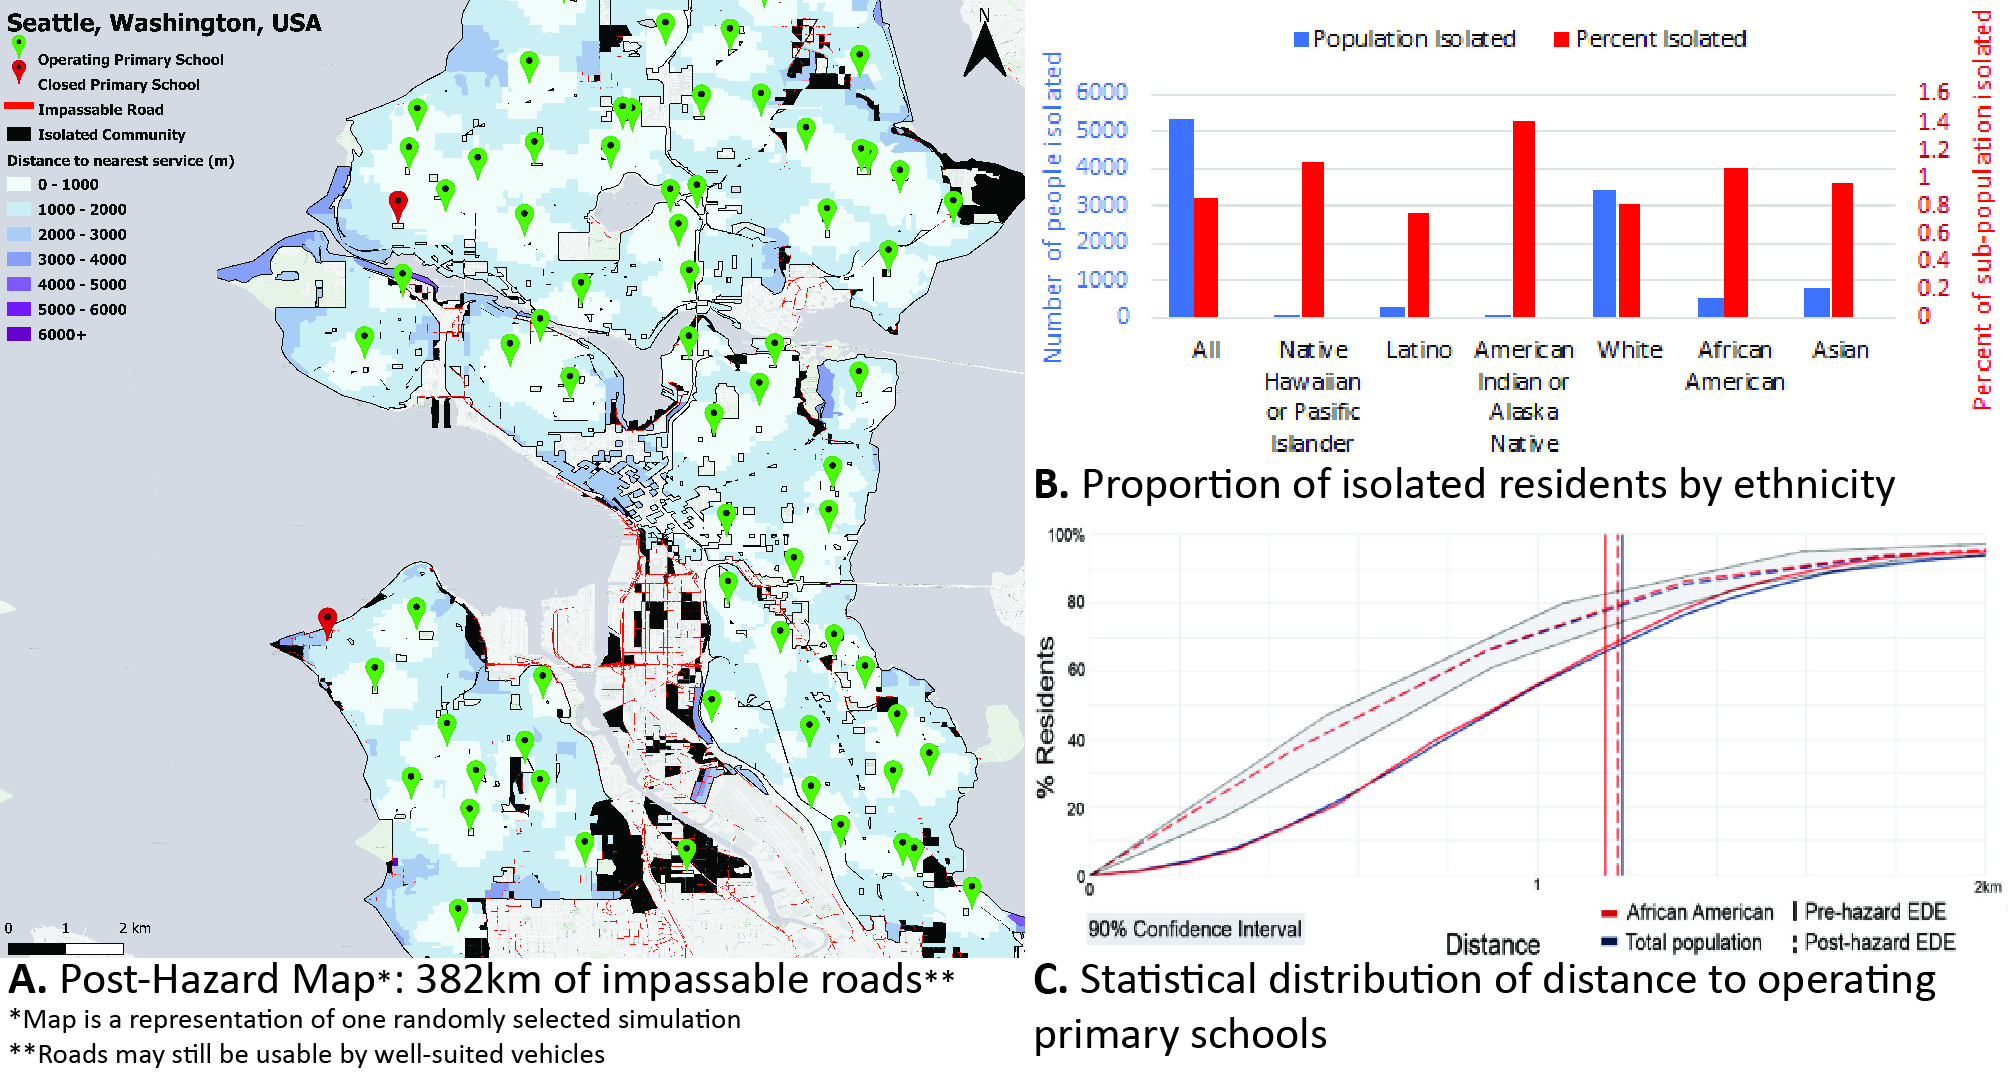
\includegraphics[width=1\linewidth]{report/fig/wa_fig.jpg}
    \caption{Evaluation of Seattle (WA, USA) access to primary schools under a liquefaction hazard scenario. \autoref{fig:seattle_fig}(a) shows a randomly selected hazard and access simulation, depicting inoperable roads \& services, isolated regions, and the level of access for the remaining population. \autoref{fig:seattle_fig}(b) shows a breakdown of ethnicity's that have been isolated. \autoref{fig:seattle_fig}(c) shows the distribution of access from 10,000 simulations with associated uncertainty. An interactive app to explore our results is available here: [Link redacted for blind review]}
    \label{fig:seattle_fig}
\end{figure*}

% post-hazard Results
After 10,000 simulations of the liquefaction hazard scenario, we observe only a slight decrease in the residents' access.
% Change in dist, change in dist for ethnicity
The averaged EDE from all 10,000 simulations was shifted upwards by 0.002km from the EDE under normal circumstances, at first glance this indicates that access has not been impacted.
However, some regions of the city have become isolated from all primary schools, this can be seen in the blacked-out regions of \autoref{fig:seattle_fig}(a). 
The distribution of ethnic groups who have been isolated can be seen in \autoref{fig:seattle_fig}(b).
Moreover, most of the damaged roads seen within \autoref{fig:seattle_fig}(a) are located within the center of the city near the port, so while residents access to primary schools is relatively unaffected, the use of the port will be severely disrupted.
% why has the cdf increased?
While several people have become isolated and the EDE has become worse, the distribution (\autoref{fig:seattle_fig}c) shows the post-hazard access distribution has been shifted up to the left.
This suggests that the access may have slightly improved.
This alleged improvement is due to the isolated residents not being included in the calculation, as their distance is infinite.
As this is weighted by population, the removal of approximately 5,000 residents who, before the hazard, would have resided at a distance greater than the initial EDE (1.88km), has caused the visual improvement of the distribution.
% equity
In terms of equity of access and isolation, the post-hazard EDE indicates continued equity for those that have access after the event.
Additionally, \autoref{fig:seattle_fig}(b) shows that all ethnicities are approximately equally represented within the isolated residents.

\subsubsection{Houston: Hurricane Inundation/Flooding}
%hazard hist, known food/health deserts, previous studies (including harvey), population etc.
For our second case study, we evaluate the access of Houston (TX, USA) residents to their nearest medical center.
Houston has been identified in multiple studies as a region with poor distributional justice and poor equitable access to various services such as supermarkets, health care, and green spaces \cite{Logan2021-ineq, Significantly2012-sr, Haefner2021-ro, The_Trust_for_Public_Land2018-cm}.
% economics - transport reliance
Being the fourth most populous city within the US, Houston is a hub for Texas and the wider southern region of the country and therefore has one of the greatest demands for a reliable transport network.

\begin{figure*}[h]
    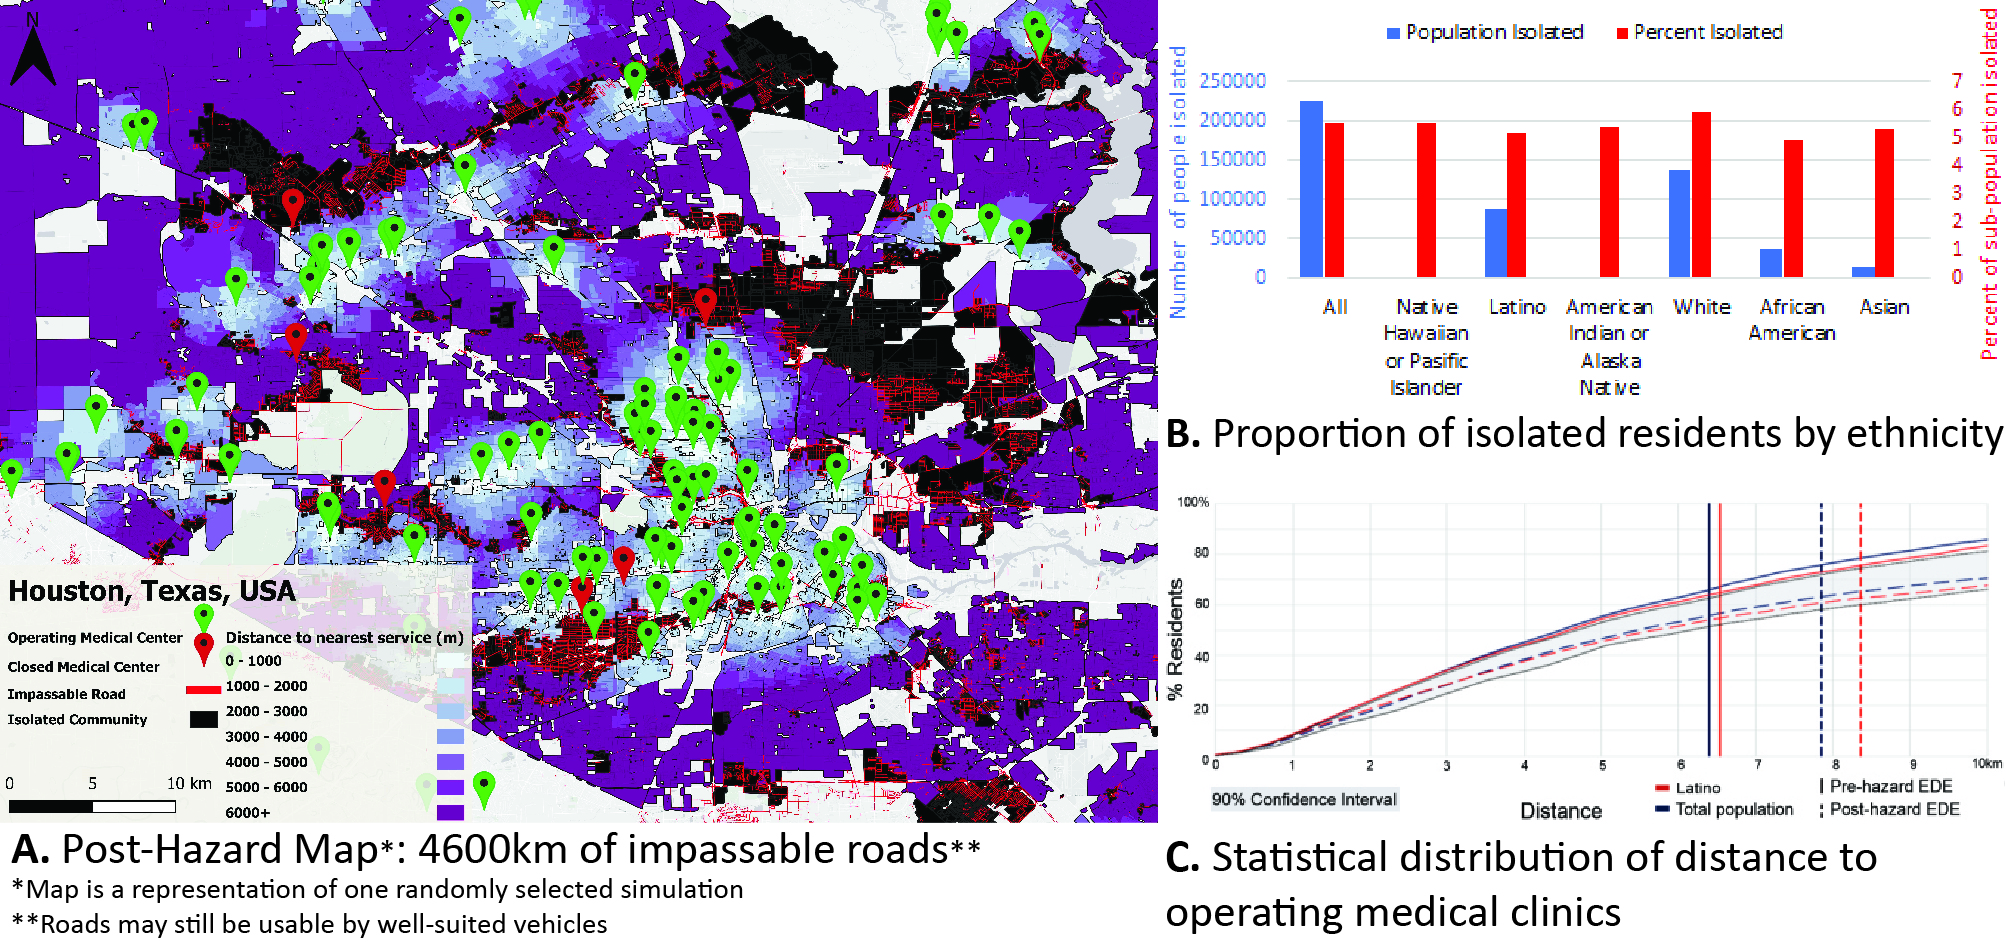
\includegraphics[width=1\linewidth]{report/fig/tx_fig.jpg}
    \caption{Evaluation of Houston (TX, USA) access to medical clinics under a hurricane inundation hazard scenario. \autoref{fig:houston_fig}(a) shows a randomly selected hazard and access simulation, depicting inoperable roads \& services, isolated regions, and the remaining populations level of access. \autoref{fig:houston_fig}(b) shows a breakdown of ethnicity's that have been isolated. \autoref{fig:houston_fig}(c) shows the distribution of access from 10,000 simulations with associated uncertainty. An interactive app to explore our results is available here: [Link redacted for blind review]}
    \label{fig:houston_fig}
\end{figure*}

Unfortunately, Houston is prone to flooding events much like Hurricane Harvey which made landfall in 2017 and flooded the city while claiming approximately 68 lives \cite{FEMA_Data}.
Using empirical inundation depth data collected from this event, we simulate the hazard on the city to understand the impacts on access.
The distribution of access prior to this simulated event can be seen in \autoref{tab: BAU_Results}, consistent with previous studies, we find that Houston has poor and inequitable access to medical clinics.
% post-hazard Results
% 1 iteration - map results
% road loss, service loss
After 10,000 simulations of this flood hazard, we see dramatic changes in the overall access distribution for the population, with an EDE shift of 1.5km and a further 220,000 residents completely isolated.
These results can be seen in \autoref{fig:houston_fig}.
Within \autoref{fig:houston_fig}(c) we see the gap between the total population EDE and the Latino EDE is significantly wider after the hazard, indicating that the Latino population is disproportionately impacted.
Lastly, in terms of isolated populations, all racial and ethnic groups are similarly impacted (\autoref{fig:houston_fig}(b)).


\subsection{Multi-Hazard Scenario}
Christchurch was chosen as an example outside of the USA and due to its exposure to a range of hazards.
It is well-studied due to the 2010-2012 Canterbury Earthquake Sequence. 
Additionally, the city has an estimated 25,000 household’s exposed to coastal inundation within the next 100 years.
It is, therefore, possible to have multiple hazards occur within similar time periods.

Current efforts to evaluate hazard exposure and subsequent risk often fail to address the concept of equality and can propose potentially maladaptive risk treatment measures by solely focusing on individual hazards or scenarios. 
Therefore, where possible we should consider not only single hazard events but also multi-hazard events.
Given the data availability for Christchurch, we have the opportunity to analyse the impacts to access under a multi-hazard scenario for an approximately 1 in 2500-year earthquake-induced tsunami event causing coastal inundation and liquefaction. 
This is completed by utilising data from \cite{Mueller2019-hk, Tonkin_taylor2020-es}.

Utilising a multi-hazard approach, although simplified for a proof of concept \cite{Gehl_undated-rx}, we can analyse the impacts and test possible interventions within each single hazard scenario and multi-hazard scenario.
The ability to test interventions across a range of scenarios limits the possibility of providing adaptation options to one hazard scenario which may worsen the impacts from another hazard scenario.

\subsubsection{Christchurch: Earthquake Induced Tsunami}
\begin{figure*}[h!]
    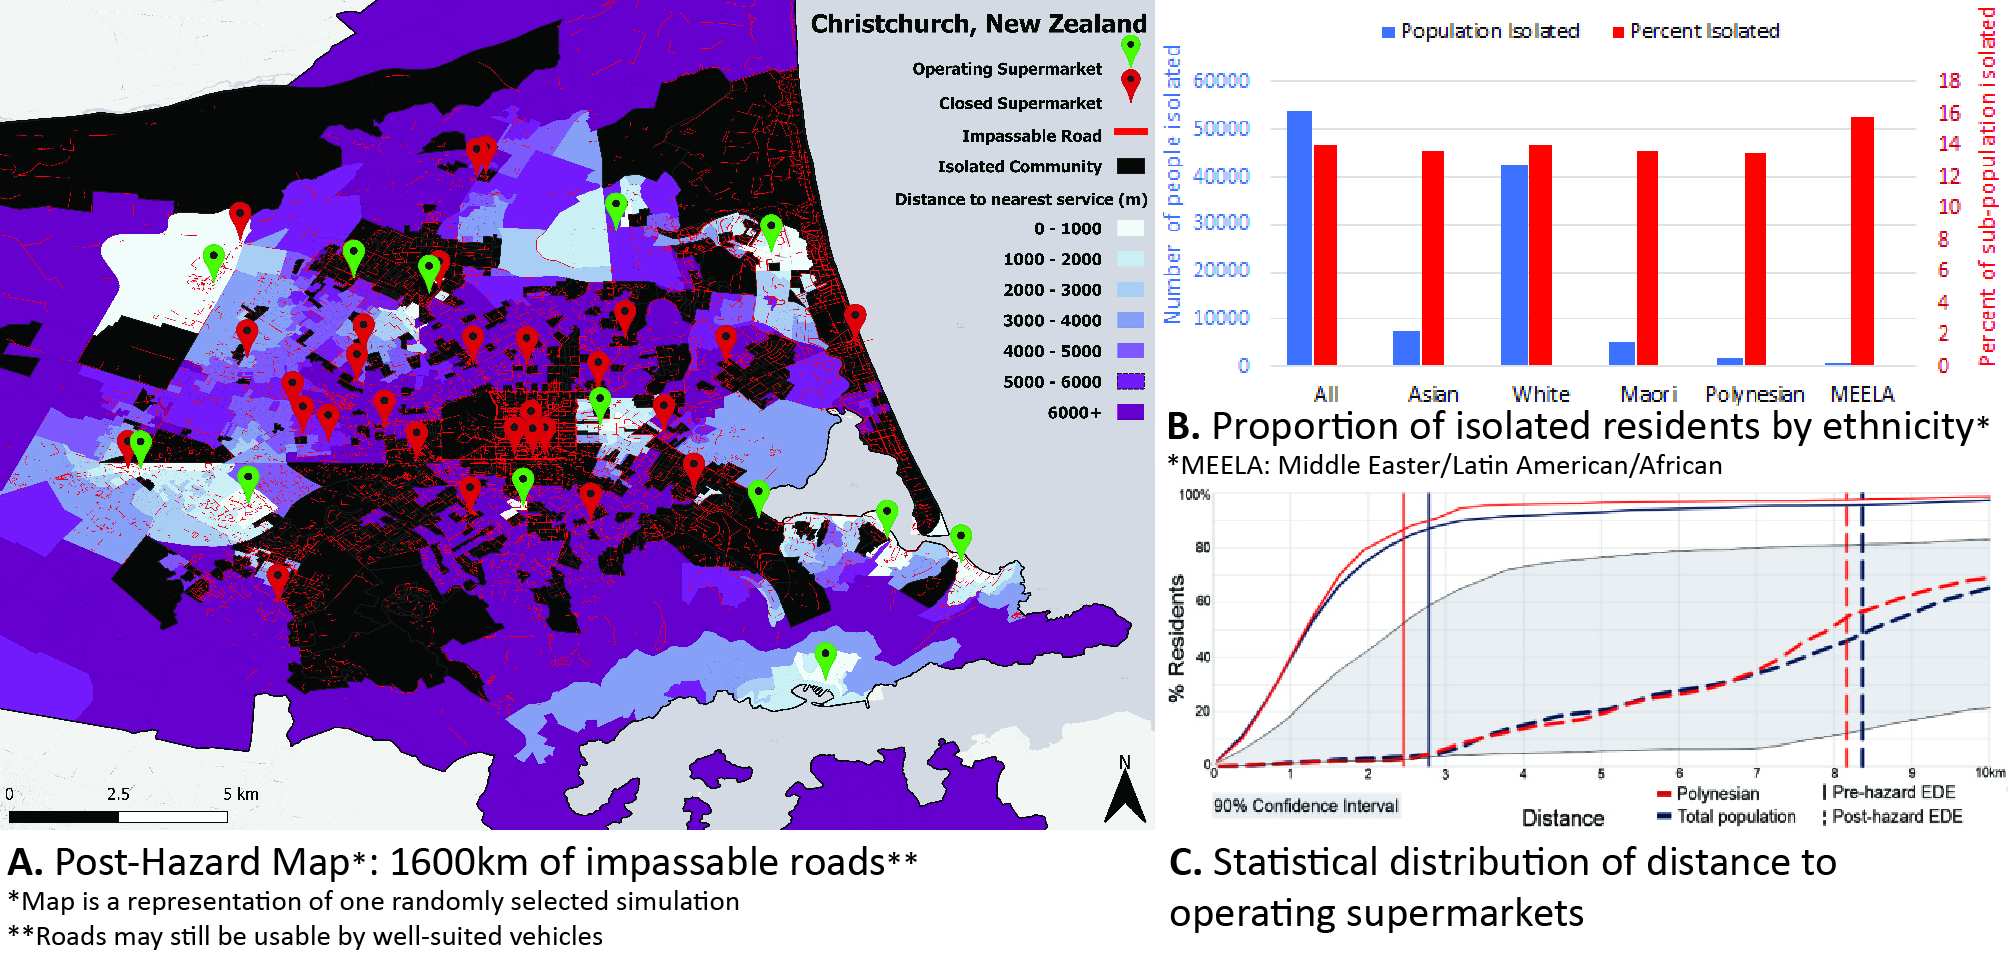
\includegraphics[width=1\linewidth]{report/fig/ch_fig.jpg}
    \caption{Evaluation of Christchurch (New Zealand) access to supermarkets under a multi-hazard scenario. \autoref{fig:chch_fig}(a) shows a randomly selected hazard and access simulation, depicting inoperable roads \& services, isolated regions, and the remaining populations level of access. \autoref{fig:chch_fig}(b) shows a breakdown of ethnicity's that have been isolated. \autoref{fig:chch_fig}(c) shows the distribution of access from 10,000 simulations with associated uncertainty. An interactive app to explore our results is available here: [Link redacted for blind review]}
    \label{fig:chch_fig}
\end{figure*}

Christchurch's access to supermarkets and the equity of such is, relative to the other cities, average \autoref{tab: BAU_Results}. 
However, after 10,000 iterations of a multi-hazard scenario, we can see in \autoref{fig:chch_fig}(c) that the EDE is shifted by 5.6km for the total population, with over 50,000 residents isolated from any supermarket facility.
Within one randomly selected simulation result, seen in \autoref{fig:chch_fig}(a), we note that over a quarter of the roads in the city have been deemed impassable and the majority of supermarkets have been closed.
We also analyse the Polynesian population within the city who have better access initially.
This rank order remains after the hazard, however, the difference in EDEs is reduced.
This indicates a larger access disruption for Polynesian residents.
Finally, when considering isolated residents, much like the other case studies, the ethnic representation within the isolated population is still equally distributed.


\subsection{Optimising Recovery Efforts}
% previous planning and recovery failures
While natural hazards don't discriminate, recovery efforts often do.
This is seen through various planning failures and disaster recovery efforts around the globe.
Examples such as the previously mentioned Hurricane Katrina and Pokeno scenario are further evidence of this.
This provides motivation to find better methods that guide decision-makers to consider equity throughout the recovery process.

\begin{figure*}[b!]
    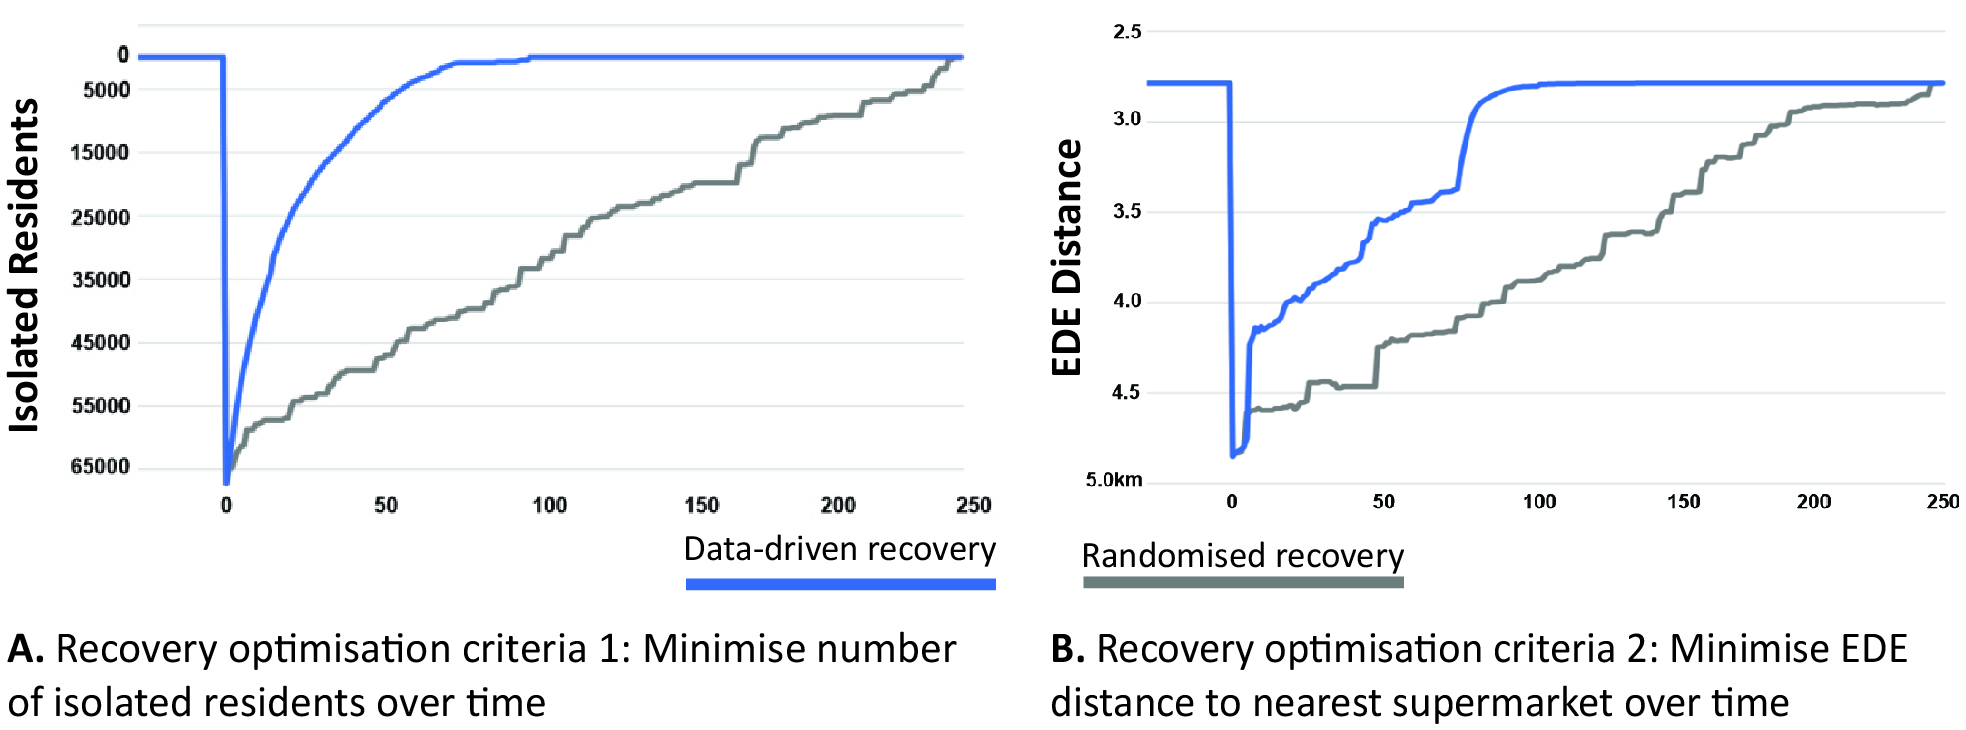
\includegraphics[width=0.95\linewidth]{report/fig/recovery_fig.jpg}
    \caption{Recovery curves for Christchurch (New Zealand) based on a simulated multi-hazard event. \autoref{fig:recovery_fig}(a) shows how the number of isolated residents can be recovered optimally. \autoref{fig:recovery_fig}(b) shows how the equitable access (EDE) can be simultaneously recovered optimally.  An interactive app to explore our results is available here: [Link redacted for blind review]}
    \label{fig:recovery_fig}
\end{figure*}

Using the approach provided within this paper to assess the indirect impacts of a hazard on the transportation network we can also test different pathways of recovery and their outcomes.
We demonstrate this in \autoref{fig:recovery_fig} where we take a randomly selected simulation result from the Christchurch liquefaction event and optimise the order of infrastructure (road segments and services) restoration.
We optimise for the maximum decrease in isolated residents followed by the maximum decrease in the EDE distance to an operable supermarket.
This creates a recovery curve that can be compared with a randomised recovery process.
\autoref{fig:recovery_fig} clearly shows the improvement of using a data-driven approach.
Had this been a real disaster, the implications of the randomised recovery compared to the optimised recovery would be huge.
It should be noted that this prioritises the order of restoration actions based on the outcome of the EDE.
In practice, this approach should be coupled with the experience of decision-makers who can assess the financial cost and time of each restoration action as well as their optimised outcomes.
This approach can be used with real-time disaster data if needed and it is also flexible to be used with different services and demographics to ensure justice within the recovery process.

%%%%%%%%%%%%%%%%%%%%%%%%%%%%%%%%%%%%%%%%%%%%%%%%%%%%%%%%%%%%%%%%%%%
% DISCUSSION
%%%%%%%%%%%%%%%%%%%%%%%%%%%%%%%%%%%%%%%%%%%%%%%%%%%%%%%%%%%%%%%%%%%
\section{Discussion}

% P1: What is the point of this paper - bring back ideas from intro
The objective of this paper is to enhance the understanding of the role of the transportation network in supporting community resilience. 
Crucial to this is improving our understanding of the indirect influences, especially in situations with disruptions.
% explore approach to evaluate direct and indirect impacts from a disruption in the transportation network
% enhance understanding of the critical role that the transportation network plays in community resilience
To achieve this, this paper outlines an approach that enables transport and urban planners to evaluate the direct and indirect impacts caused by a disruption within the transportation network.
% The ability to evaluate these indirect impacts enhances our understanding of the critical yet, occasionally underestimated role that the transportation network plays in community resilience.

% P2: Proposed (fine resolution) approach lets us firstly explore the direct impacts
% direct impacts
% results
One of the benefits of the approach is the high spatial resolution that allows us to examine the direct impacts that a hazard may have on individual elements of the transportation network and then determine the subsequent impact on the wider network.
These direct impacts include the spatial distribution of damaged roads as well as damaged amenities, which ultimately, the transport network exists to connect people to.
For example, within our liquefaction scenario in Seattle, we see a small number of services and approximately 5\% of the road network close.
We also use this approach in Christchurch under a multi-hazard scenario and can quickly identify the direct impacts: over a quarter of the roads within the city are impassable and over 65\% of the supermarkets were deemed inoperable.

% P3: Also lets us explore indirect impacts
% access & equity
Beyond the direct impacts, we can explore the indirect impacts that result from closed services and transport routes.
In the case of Seattle, while we noted very little change in access for residents to primary schools, the majority of damaged roads were located by the port.
Given that Washington state ranks among the highest in the country in per capita exports, this event could have major consequences on the city and its economy \cite{McNamee2016-ms}.
Another example is provided in Houston (TX, USA) which sees direct impacts of 8\% and 7.5\% closures within the road network and medical centers respectively.
This has significant implications on the city's residents.
Specifically, Houston residents would have to travel, on average, 8km to their nearest health care provider.
This increases the vehicle dependence within the city and therefore increases the contribution to the city's transport emissions.

Of more pressing concern in disaster scenarios, are the disproportionate impacts on the residents, which our approach enables us to explore.
% % equity
% However, understanding the change in access must be done in conjunction with equity.
% Using this approach we can then explore the change in equity among residents.
We demonstrate this potential with an analysis of the equity of access between ethnic groups.
Continuing with the results of the Houston case study we see that under normal circumstances the Latino population has comparable proximity to their nearest medical center when compared with the rest of the city.
However, after a flooding event, the average distance that a Hispanic/Latino resident must travel to a health care facility is over half a kilometer further than the rest of the population.
This is of particular importance for low-income or non-car owning individuals who may be disproportionately impacted in the event of a disaster \cite{cutter2003social, Frazier2013-wd, Sherrieb2010-lk}

% P4: Exploring indirect impacts
% isolation
Furthermore, this approach enables us to identify residents and areas within a city that are at risk of becoming isolated from certain services after a hazard event.
For example, while an earthquake in Seattle has minor direct impacts on the road network, we reveal that potentially 5,000 residents may be isolated from all primary schools. 
Potentially of more pressing concern is that we identify that 220,000 residents could be isolated from health care within the Houston flooding scenario.
Isolation from services such as education, food, or health care has major implications on the individuals affected and violates the human right to adequate housing \cite{Cutter2003-xi, Frazier2013-wd}
This risk of isolation also has serious implications if people need to evacuate, be rescued, or receive emergency care. 
The question of equity can also be raised among isolated residents, where our approach enables users to evaluate the percentage representation of different ethnicities within the isolated population.
% Across all three of our case studies, each ethnic group was represented relatively equally, suggesting that in some cases equity is only lost during recovery interventions.

% insight
% cities with better initial access (and equity) typically have a lower percentage change in access
These results suggest that cities with initially poor access and poor access equality, are often the ones whose residents will be impacted disproportionately when compared with cities that have higher, more equitable access.
This is motive for city and transport planners to integrate measures of access and equity when evaluating potential development.
We also see more explicitly just how (and where) the transport network can make or break community resilience by inhibiting or allowing residents to access the services they need.

% P5: Benefits of the approach
% (in)direct impacts
% computationally feasable 
% open source data
% multi-hazard
Because the approach is computationally feasible (which will only improve in future), it enables researchers and practitioners to use this approach to foster access resilience and, subsequently, community resilience.
The majority of the required data is openly available and our examples demonstrate that risk and hazard assessments can be done by using both single and multi-hazard approaches.
This reduces the chance of maladaptive policy or action, and the results of such assessments with this approach enhances our understanding of transport's role in community resilience.


% P6: Therefore, should be used by TPs to enhance understanding
% Scenario planning & investment
% lifeline road identification
Furthering our understanding and enhancement of community resilience in relation to the transport network, this tool can be used for scenario planning to identify critical or lifeline transport routes and services.
By understanding where the likely areas of major access disruption or isolation are, we can guide investment decisions towards a more reliable and robust transportation system.
The benefits are two-fold by both increasing the likelihood that communities can continue to function in the event of a natural hazard as well as improving general access and access equality. 
Both have wider community benefits \cite{logan2020reframing, Frazier2013-wd}. 
% This, of course, makes our communities more resilient by allowing continued community function through access to different resources, services, and amenities.



% P8: Use by TPs and others
% Emergency management training and community engagement
This approach can also be used for training emergency managers and key decision-makers in a community. 
% approach to enhance the intuition and knowledge of emergency managers and individuals within the community.
This can be achieved by using the simulation approach in emergency management training where users can build intuition and understanding of the indirect impacts and implications of equity and access throughout the recovery process.
We are in the process of implementing this tool to be suitable for community engagement on coastal hazards adaptation planning to assist residents to both evaluate future scenarios and interventions, as well as to enable them to better prepare and evaluate their readiness for disasters.
% For community members, this approach can be used as an interactive educational tool where residents can understand what the impacts may be to them if a hazard were to occur.
% This enables residents to 


% P9: Use by Tps and others
% recovery optimisation
% avoiding past failures of poor planning and recovery
Finally, this approach can be used to avoid past planning and recovery failures like those described earlier in Pokeno and New Orleans.
Instead, we can use this approach to guide equitable recovery.
The enhancement that this restoration approach can make to community function is evident within \autoref{fig:recovery_fig}.
Future work could couple this method with real-time outage data to provide a prioritised list of restoration actions that will maximise the number of people that access is restored equitably.


%%%%%%%%%%%%%%%%%%%%%%%%%%%%%%%%%%%%%%%%%%%%%%%%%%%%%%%%%%%%%%%%%%%
% CONCLUSION
%%%%%%%%%%%%%%%%%%%%%%%%%%%%%%%%%%%%%%%%%%%%%%%%%%%%%%%%%%%%%%%%%%%

\section{Conclusion}
% The contribution of this paper is...
With 70\% of the world's population projected to live in cities by 2050, understanding community resilience is critical to the successful future of our urban environments.
Without adequate and equitable access to resources and opportunities communities will struggle to adapt to and recover from the physical pressures being placed upon them.
Within this paper, we further the understanding of community resilience by providing an approach that highlights the importance of the transportation network.
We do this by evaluating the direct and indirect impacts on communities after a disruption in the transportation network.
Specifically, we consider how access and equity of access to key services changes over the time frame of a disaster.
This approach is demonstrated in three case studies where it was seen that the initially equal access communities can become disparate after a hazard, disproportionately impacting minority or vulnerable populations.
Demonstrating the approach’s functionality with the three case studies determined that cities with robust and equitable initial access are likely to be more resilient to the shock imposed by a natural hazard. 

Our approach leverages the recent advances in data availability and computational power which makes repeatedly simulating damage and disruption, at the link level, practicable.
This ultimately enables transport \& urban planners, and emergency managers to consider the wider implications of the transport network.
That is, we can consider how disruptions to roads and destinations will impact residents spatially throughout the city.

There are exciting opportunities for the future progress of this approach by incorporating interdependent infrastructure analysis.
This approach will open up new avenues to aid with equitable and effective climate change adaptation within our cities.
It can do this by improving the measurement of indirect impacts and the understanding of the effects that they will have on community resilience.
Improvements in access will begin to increase the health, well-being, safety, and livability of our cities.
Therefore, we urge transport planners to integrate measures of access and equity to key services into their future work to ensure that community resilience is being enhanced.

% \backmatter

% \section*{Acknowledgment}
% We would like to thank QuakeCoRE and the University of Canterbury for their support during the period of research. Respectively they provided 3 months funding to begin this research and a UC Doctoral Scholarship to continue and complete this work.

\printbibliography

\clearpage
\newpage
% \linenumbers
\appendix
%%%%%% %%%%%%%%%% %%%%%%%%%% %%%%%%%%% %%%%% SUPPLEMENTAL %%%%%%%%% %%%%%%%%%% %%%%%%%% %%%%%%%%

\section{Technical guide}

% \subsection{}
\noindent Code is available at [Link redacted for blind review] %\url{https://github.com/urutau-nz/access_resilience}.

\noindent An interactive app to explore results is available at [Link redacted for blind review]


\clearpage
\section{Supporting material}

\begin{table}[h!]
\small
\caption{Fragility thresholds for infrastructure under different hazard scenarios and exposure levels}
\begin{center}
\label{tab: fragility}
\begin{tabular}{ c|c|c|c|c } 
% \hline
Infrastructure Type & Hazard Type & Hazard Intensity & Exposure Level & Probability of closure \\ 
\hline
\multirow{9}{4em}{Road} & \multirow{3}{4cm}{Hurricane Inundation} & $\leq$ 0.3m & Low & 0\% \\ 
& & $>$ 0.3m & High & 100\% \\ 
\cline{2-5}
& \multirow{3}{4cm}{Tsunami} & 0.25m - 0.5m & Low & 10\% \\ 
& & 0.5m - 2m & Medium & 40\% \\ 
& & $\geq$ 2m & High & 80\% \\ 
\cline{2-5}
& \multirow{3}{4cm}{Liquefaction} & - & Low & 5\% \\ 
& & - & Medium & 30\% \\ 
& & - & High & 75\% \\ 
\cline{2-5}
& \multirow{3}{4cm}{Earthquake Induced Tsunami (multi-hazard scenario)} & - & Low & 15\% \\ 
& & - & Medium & 50\% \\ 
& & - & High & 90\% \\ 
& & - & Very High & 100\% \\ 
\hline
\multirow{9}{4em}{Building} & \multirow{3}{4cm}{Hurricane Inundation} & $\leq$ 2.2m & Low & 10\% \\ 
& & 2.2m - 7m & Medium & 50\% \\ 
& & $\geq$ 7m & High & 90\% \\ 
\cline{2-5}
& \multirow{3}{4cm}{Tsunami} & $\leq$ 0.5m & Low & 40\% \\ 
& & 0.5m - 2m & Medium & 80\% \\ 
& & $\geq$ 2m & High & 97.5\% \\ 
\cline{2-5}
& \multirow{3}{4cm}{Liquefaction} & - & Low & 10\% \\ 
& & - & Medium & 33\% \\ 
& & - & High & 80.5\% \\ 
\cline{2-5}
& \multirow{3}{4cm}{Earthquake Induced Tsunami (multi-hazard scenario)} & - & Low & 45\% \\ 
& & - & Medium & 85\% \\ 
& & - & High & 97.5\% \\ 
& & - & Very High & 100\% \\ 
% \hline
\end{tabular}
\end{center}
\end{table}


\begin{table}[h!]
\small
\caption{Data Sources}
\begin{center}
\label{tab: data}
\begin{tabular}{p{2cm}|p{2cm}|p{4cm}|p{3cm}|p{3cm}}%{ c|c|c|c|c } 
\small
% \hline
Data & Location & Comment & Source & Reference \\ 
\hline
Transportation Networks & All & - & OpenStreetMap via OSMNX & \cite{OpenStreetMap, Boeing2017-nf} \\
\hline
Origins \& Demographics & Christchurch & Statistical Area 1 & Stats NZ & \cite{Stats_NZ} \\
\hline
Origins \& Demographics & Seattle \& Houston & Census Block & TIGER/Line & \cite{census:2011} \\
\hline
Boundary & Christchurch & - & Christchurch City Council & \cite{Stats_NZ} \\
\hline
Boundary & Seattle & King County & - & - \\
\hline
Boundary & Houston & Harris County & - & - \\
\hline
Destinations & Christchurch & Supermarkets & OpenStreetMap via OverPassTurbo & \cite{OpenStreetMap} \\
\hline
Destinations & Seattle & Primary Schools & National Center for Education Statistics & \cite{National_Center_for_Educational_Statistics2020-zk} \\
\hline
Destinations & Houston & Medical Centers & OpenStreetMap via OverPassTurbo & \cite{OpenStreetMap} \\
\hline
Hazard: Tsunami & Christchurch & 1 in 2500 year event & Institute of Geological and Nuclear Sciences (GNS) & \cite{Mueller2019-hk} \\
\hline
Hazard: Liquefaction & Christchurch & Liquefaction susceptibility map under a magnitude 6.0 earthquake & Tonkin \& Taylor & \cite{Tonkin_taylor2020-es} \\
\hline
Hazard: Liquefaction & Seattle & Relative liquefaction susceptibility & United States Geological Survey (USGS) & \cite{palmer2004liquefaction} \\
\hline
Hazard: Hurricane Inundation & Houston & Empirical data from Hurricane Harvey & FEMA & \cite{FEMA_Data} \\
% \hline
\end{tabular}
\end{center}
\end{table}


\renewcommand\thefigure{A.\arabic{figure}} 

\end{document}


